% Playbook schematic, revised 7 October 2026 from Aimee Harrison's draft of
% 6 October (the unchanged original is kept at
% manuscript/.build/overleaf-fresh-20261007-schematic.tex). Two revision
% rounds: an initial rewrite, then corrections from a read-only Codex
% adversarial review (.turbo/codex/schematic-review.txt).
%
% What changed from the 6 October draft, and why:
%  1. Numbering follows the manuscript's Steps 0 to 6. The draft's Phase labels
%     did not map onto those Steps (discovery sat before "Phase 2" although it is
%     Step 2; "Phase 4" mixed Step 4's game construction with Step 5's
%     attribution), so the mapping footnote was removed rather than kept.
%  2. Core principle: cross-algorithm agreement on one dataset is limited
%     robustness evidence under explicit, different assumptions; it is not
%     independent validation. Validity rests on testable implications (with
%     rejection as the informative outcome), edge evidence from outside the
%     dataset, and sensitivity of the target to the alternatives still open.
%  3. Discovery: "keep edges both support" (intersection) replaced by keeping
%     each candidate graph or equivalence class with its provenance. A set union
%     is not used either: it need not be acyclic or orientation-consistent.
%     Aggregation, if wanted, uses a defined ensemble or validation procedure.
%  4. A supplied, fully specified DAG enters review directly, as the manuscript
%     and supplement state; diagnostic discovery is optional.
%  5. Target routes: an intervention question goes to identification under
%     stated assumptions and then to an estimator (g-computation, IPW, TMLE);
%     allocation is optional. Allocation declares its game (value function,
%     players, order law or allocation rule, background, scale) in Step 4 and
%     computes in Step 5. The undefined labels "Causal Interventional SHAP" and
%     "Causal Predictive SHAP" are gone.
%  6. Review of results checks each result against its own target and support
%     conditions; disagreement across games is expected, not a failure signal.
%     Positivity is defined for a target, population and required support, not
%     for "sparse nodes" in general.
%  7. Step 6 has three exits (resolved, revise, unresolved) and the graph-only
%     route reaches the review and report, so no branch dead-ends.
%  8. Rules rewritten with citations whose scope matches each sentence; the
%     small-sample claim is withdrawn until the degradation experiment runs;
%     per-item daggers are replaced by one scope statement.
%
% Build (from this folder): pdflatex, bibtex, pdflatex, pdflatex.
\documentclass[10pt,a4paper]{article}
\usepackage[utf8]{inputenc}
\usepackage[T1]{fontenc}
\usepackage[margin=0.65in]{geometry}
\usepackage{tikz}
\usepackage{float}
\usepackage{adjustbox}
\usepackage[numbers,sort&compress]{natbib}
\usepackage[hidelinks]{hyperref}
\usetikzlibrary{shapes.geometric, arrows.meta, positioning, calc}

\title{\Large\textbf{Playbook: Graph Construction, Review, and Causal Attribution}}
\author{\small\textbf{A Decision Guide for the Causal Modeling Pipeline}}
\date{\small Revised 7 October 2026}

% Compact TikZ style definitions (box widths enlarged from the 6 October draft)
\tikzstyle{startstop} = [
  rectangle,
  rounded corners,
  minimum width=3.3cm,
  minimum height=0.75cm,
  text centered,
  draw=black,
  fill=white,
  text=black,
  text width=3.2cm,
  font=\scriptsize\bfseries
]

\tikzstyle{process} = [
  rectangle,
  minimum width=3.4cm,
  minimum height=0.7cm,
  text centered,
  text width=3.3cm,
  draw=black,
  fill=white,
  text=black,
  font=\scriptsize
]

\tikzstyle{review} = [
  process,
  draw=black,
  line width=1.1pt,
  fill=black!8
]

\tikzstyle{decision} = [
  diamond,
  minimum width=2.2cm,
  minimum height=0.8cm,
  text centered,
  text width=2.0cm,
  draw=black,
  fill=white,
  text=black,
  font=\scriptsize,
  inner sep=1pt
]

\tikzstyle{arrow} = [thick, ->, >=stealth]

\begin{document}

\maketitle
\vspace{-0.6cm}

\section*{Scope \& Prerequisites}
\small \textbf{Scope:} Assumes a dataset in which the variables of interest are measured and in which selection into the dataset can be represented. Dataset identification and raw ETL are out of scope. The steps are the manuscript's Steps~0--6.

\noindent\textbf{Core principle:} No single analysis establishes a DAG or an attribution. Confidence in a graph comes from its testable implications and from evidence about its edges gathered outside the dataset. It also depends on how much the target changes across the alternatives still open. Agreement between algorithms run on one dataset can be limited robustness evidence when their assumptions differ; it is not independent validation of the graph. Every branch ends in expert review.

\noindent\textbf{Status of these recommendations:} They rest on reasoning and the cited literature. The accompanying simulation study tested none of them except where a record is named in the text.

\section*{Key Execution Rules \& Safeguards}
\begin{enumerate}\small
    \item \textbf{Triangulate; Do Not Duplicate:} Pair a method with one whose main sources of bias differ, or with evidence from outside the dataset (experiments, timing, mechanism) \citep{Lawlor2016,MunafoDaveySmith2018}. Agreement between algorithms run on the same data cannot detect shared measurement, selection or omitted-variable error, and benchmark success can come from a shared artifact such as variance ordering \citep{Reisach2021}. Where aggregation is wanted, use a defined ensemble or validation procedure rather than a vote \citep{Viinikka2018,Chowdhury2022}.
    \item \textbf{Report Structural Uncertainty; Do Not Merge Graphs by Hand:} Keep each candidate graph or equivalence class with its provenance. A set union of outputs need not be acyclic or orientation-consistent, and an intersection cannot raise recall; it only removes edges. Markov-and-faithfulness methods such as PC and GES return an equivalence class, so report the set of effects compatible with it \citep{Spirtes2000,Maathuis2009}; functional methods such as LiNGAM can identify a DAG under stronger assumptions \citep{Shimizu2006}. Edge frequencies from resampling measure the stability of the fitted procedure, not causal confidence \citep{Friedman1999,ScutariNagarajan2013}. Match tests to the variable types \citep{Sedgewick2019,Tsagris2018}; the renal Gaussian-PC run that found no outcome adjacency is a mixed-data diagnostic awaiting follow-up.
    \item \textbf{Test Implications; Rejection Is the Informative Outcome:} The conditional independencies a graph implies are its testable content \citep{Textor2016,Ankan2021}. Prespecify them and test on held-out or external data where possible. Rejection challenges the graph or the test's assumptions; non-rejection is not confirmation. Report multiplicity, the test's assumptions and power against relevant departures: no conditional-independence test is uniformly valid without assumptions \citep{ShahPeters2020}, near-faithfulness violations and finite power make weak dependencies hard to detect \citep{Uhler2013,ZhangSpirtes2003}, and tests run on the data that selected the graph need post-selection handling \citep{Chang2026}.
    \item \textbf{Represent Selection Explicitly:} Add a selection indicator with arrows from its causes and represent the analyzed cohort as conditioned on that indicator. Some implications of a correct DAG then fail for that reason alone \citep{HernanSelection2004}.
    \item \textbf{Positivity Belongs to the Target, Not to Node Depth:} Positivity is defined for a specified intervention, population and required support \citep{Petersen2012,WestreichCole2010}. Where support is absent the contrast is not identified; where data are sparse the estimate is imprecise; predictive SHAP stays computable for a rare feature but is unstable. Report support diagnostics for each method and estimand.
    \item \textbf{Declare the Game Before Reading the Number:} An attribution answers the question its value function asks: conditional, model-interventional, outcome-based do-Shapley, or a fitted-model interventional analogue, each with its players, order law or allocation rule, background and scale \citep{Janzing2020,Heskes2020,Jung2022,Frye2020,Wang2021}. In this study's matched comparison, ordering alone produced no detected improvement. The oracle-mechanism prototype changed both the value function and the order law; its larger agreement is provisional and does not isolate which change caused it.
    \item \textbf{Causal Inputs Carry Their Errors Forward:} Each family consumes different causal information: an ordering for asymmetric Shapley values \citep{Frye2020}, edge structure for Shapley Flow \citep{Wang2021}, identified interventional distributions or fitted conditionals for causal Shapley and do-Shapley \citep{Heskes2020,Jung2022}, and supplied mechanisms for the propagation prototype. Errors in those inputs enter the attributions, so report results across the retained graphs. No claim about small samples is made until the degradation experiment runs.
    \item \textbf{Expert Review Closes Every Branch:} This is the paper's proposed governance rule. The domain team reviews structure and results together, keeps a ledger of what changed and why, and returns unresolved disagreement to Step~3. NASA's diagramming practice supplies the configuration-management precedent \citep{Antonsen2024} and its evidence levels grade the edges \citep{Ward2024,Reynolds2022}. Where a simulation truth exists, Step~6 evaluates performance against it; success against a simulation oracle does not validate the graph for astronauts.
\end{enumerate}

\clearpage
\begin{figure}[H]
\centering
\begin{adjustbox}{max width=\textwidth, max height=0.92\textheight}
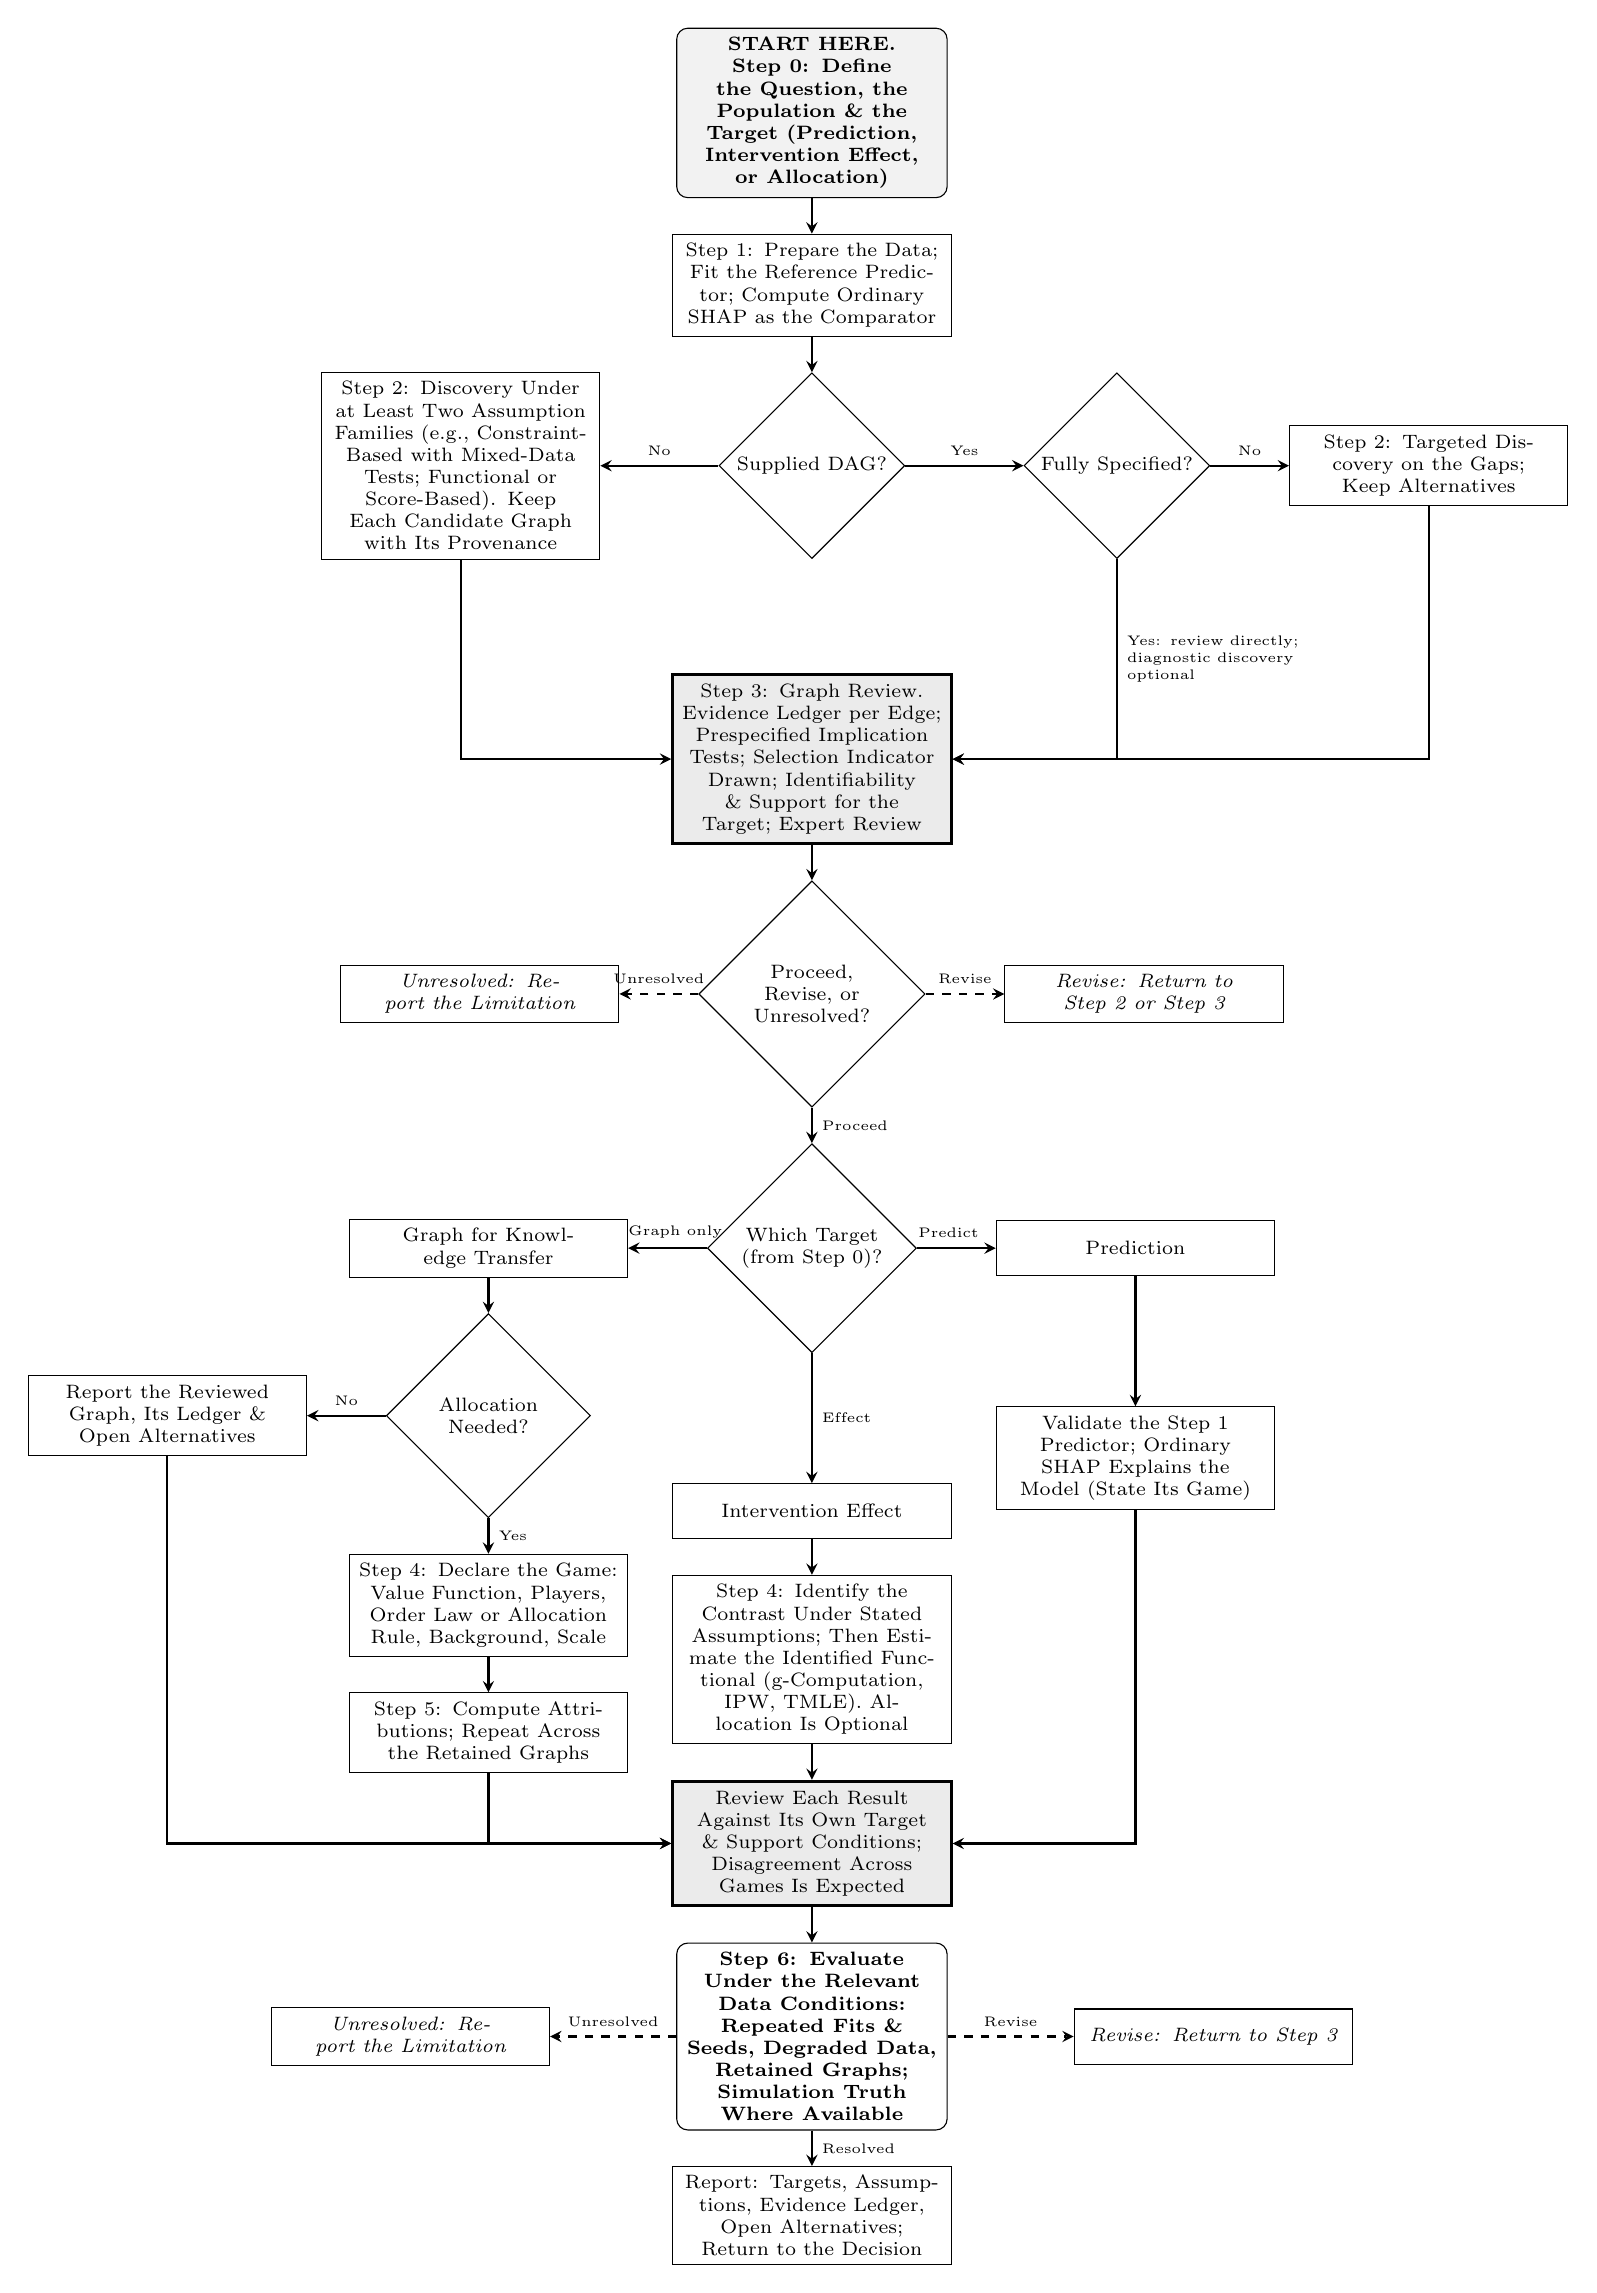
\begin{tikzpicture}[node distance=0.45cm and 1.0cm, auto]

  % --- Entry: Steps 0 and 1 ---
  \node (entry) [startstop, fill=black!5] {START HERE. Step~0: Define the Question, the Population \& the Target (Prediction, Intervention Effect, or Allocation)};
  \node (step1) [process, below=of entry] {Step~1: Prepare the Data; Fit the Reference Predictor; Compute Ordinary SHAP as the Comparator};

  % --- Step 2: graph source ---
  \node (dag_q) [decision, below=of step1] {Supplied DAG?};

  \node (discovery) [process, left=of dag_q, xshift=-0.5cm] {Step~2: Discovery Under at Least Two Assumption Families (e.g., Constraint-Based with Mixed-Data Tests; Functional or Score-Based). Keep Each Candidate Graph with Its Provenance};

  \node (spec_q) [decision, right=of dag_q, xshift=0.5cm] {Fully Specified?};
  \node (partial_disc) [process, right=of spec_q] {Step~2: Targeted Discovery on the Gaps; Keep Alternatives};

  % --- Step 3: review ---
  \node (step3) [review, below=of dag_q, yshift=-1.0cm] {Step~3: Graph Review. Evidence Ledger per Edge; Prespecified Implication Tests; Selection Indicator Drawn; Identifiability \& Support for the Target; Expert Review};

  \node (conf_dag) [decision, below=of step3] {Proceed, Revise, or Unresolved?};
  \node (revise_a) [process, right=of conf_dag, font=\scriptsize\itshape] {Revise: Return to Step~2 or Step~3};
  \node (unres) [process, left=of conf_dag, font=\scriptsize\itshape] {Unresolved: Report the Limitation};

  % Lines for Steps 0 to 3
  \draw [arrow] (entry) -- (step1);
  \draw [arrow] (step1) -- (dag_q);
  \draw [arrow] (dag_q) -- node[above, font=\tiny] {No} (discovery);
  \draw [arrow] (dag_q) -- node[above, font=\tiny] {Yes} (spec_q);
  \draw [arrow] (spec_q) -- node[above, font=\tiny] {No} (partial_disc);
  \draw [arrow] (spec_q.south) |- node[pos=0.25, right, font=\tiny, text width=2.2cm] {Yes: review directly; diagnostic discovery optional} (step3.east);
  \draw [arrow] (partial_disc.south) |- (step3.east);
  \draw [arrow] (discovery.south) |- (step3.west);
  \draw [arrow] (step3) -- (conf_dag);
  \draw [arrow, dashed] (conf_dag) -- node[above, font=\tiny] {Revise} (revise_a);
  \draw [arrow, dashed] (conf_dag) -- node[above, font=\tiny] {Unresolved} (unres);

  % --- Steps 4 and 5 by target ---
  \node (target_q) [decision, below=of conf_dag] {Which Target (from Step~0)?};

  \node (know) [process, left=of target_q] {Graph for Knowledge Transfer};
  \node (effect) [process, below=of target_q, yshift=-1.2cm] {Intervention Effect};
  \node (pred) [process, right=of target_q] {Prediction};

  \node (attr_q) [decision, below=of know] {Allocation Needed?};
  \node (pub_dag) [process, left=of attr_q] {Report the Reviewed Graph, Its Ledger \& Open Alternatives};
  \node (game) [process, below=of attr_q] {Step~4: Declare the Game: Value Function, Players, Order Law or Allocation Rule, Background, Scale};
  \node (attr) [process, below=of game] {Step~5: Compute Attributions; Repeat Across the Retained Graphs};

  \node (effect_box) [process, below=of effect] {Step~4: Identify the Contrast Under Stated Assumptions; Then Estimate the Identified Functional (g-Computation, IPW, TMLE). Allocation Is Optional};
  \node (pred_box) [process, below=of pred, yshift=-1.2cm] {Validate the Step~1 Predictor; Ordinary SHAP Explains the Model (State Its Game)};

  \node (attr_rev) [review, below=of effect_box] {Review Each Result Against Its Own Target \& Support Conditions; Disagreement Across Games Is Expected};

  % --- Step 6 and exits ---
  \node (step6) [startstop, below=of attr_rev] {Step~6: Evaluate Under the Relevant Data Conditions: Repeated Fits \& Seeds, Degraded Data, Retained Graphs; Simulation Truth Where Available};
  \node (report) [process, below=of step6] {Report: Targets, Assumptions, Evidence Ledger, Open Alternatives; Return to the Decision};
  \node (revise6) [process, right=of step6, xshift=0.6cm, font=\scriptsize\itshape] {Revise: Return to Step~3};
  \node (unres6) [process, left=of step6, xshift=-0.6cm, font=\scriptsize\itshape] {Unresolved: Report the Limitation};

  % Lines for Steps 4 to 6
  \draw [arrow] (conf_dag) -- node[right, font=\tiny] {Proceed} (target_q);
  \draw [arrow] (target_q) -- node[above, font=\tiny, pos=0.4] {Graph only} (know);
  \draw [arrow] (target_q) -- node[right, font=\tiny] {Effect} (effect);
  \draw [arrow] (target_q) -- node[above, font=\tiny, pos=0.4] {Predict} (pred);

  \draw [arrow] (know) -- (attr_q);
  \draw [arrow] (attr_q) -- node[above, font=\tiny] {No} (pub_dag);
  \draw [arrow] (attr_q) -- node[right, font=\tiny] {Yes} (game);
  \draw [arrow] (game) -- (attr);

  \draw [arrow] (effect) -- (effect_box);
  \draw [arrow] (pred) -- (pred_box);

  \draw [arrow] (attr.south) |- (attr_rev.west);
  \draw [arrow] (pub_dag.south) |- (attr_rev.west);
  \draw [arrow] (effect_box) -- (attr_rev);
  \draw [arrow] (pred_box.south) |- (attr_rev.east);
  \draw [arrow] (attr_rev) -- (step6);

  \draw [arrow] (step6) -- node[right, font=\tiny] {Resolved} (report);
  \draw [arrow, dashed] (step6) -- node[above, font=\tiny] {Revise} (revise6);
  \draw [arrow, dashed] (step6) -- node[above, font=\tiny] {Unresolved} (unres6);

\end{tikzpicture}
\end{adjustbox}

\vspace{0.1cm}
{\scriptsize Shaded boxes with heavy borders are review steps. Step numbers are the manuscript's Steps 0--6. The prediction route does not require Steps~4--5; an effect-only analysis can omit Step~5.}
\end{figure}

\bibliographystyle{unsrtnat}
\bibliography{references}

\end{document}
